\documentclass[11pt]{article}
\usepackage[paperwidth=13.333in,paperheight=7.5in,margin=0.25in]{geometry}
\pagestyle{empty}
\usepackage{tikz}
\usetikzlibrary{arrows.meta,positioning,fit,calc,shapes.geometric,backgrounds}
\usepackage{xcolor}
% The default palette is the white-background evidence-report style. The
% figure builder defines \DARKTHEME for slide-ready variants.
\ifdefined\DARKTHEME
\definecolor{ink}{HTML}{F3F7FA}
\definecolor{muted}{HTML}{B9C7D4}
\definecolor{grid}{HTML}{2B3B4B}
\definecolor{blue}{HTML}{62B8FF}
\definecolor{teal}{HTML}{55D6C2}
\definecolor{orange}{HTML}{FFBD5A}
\definecolor{red}{HTML}{FF7568}
\definecolor{purple}{HTML}{C3A6FF}
\definecolor{paleBlue}{HTML}{14283A}
\definecolor{paleOrange}{HTML}{3A2B14}
\definecolor{dataFill}{HTML}{241C3A}
\definecolor{modelFill}{HTML}{12352F}
\definecolor{specialistFill}{HTML}{3A2B14}
\definecolor{futureFill}{HTML}{1C2630}
\definecolor{pageBg}{HTML}{080D13}
\else
\definecolor{ink}{HTML}{102A43}
\definecolor{muted}{HTML}{52606D}
\definecolor{grid}{HTML}{D9E2EC}
\definecolor{blue}{HTML}{1976A8}
\definecolor{teal}{HTML}{16817A}
\definecolor{orange}{HTML}{D9822B}
\definecolor{red}{HTML}{C05640}
\definecolor{purple}{HTML}{6B5B95}
\definecolor{paleBlue}{HTML}{E8F1F5}
\definecolor{paleOrange}{HTML}{FFF1DF}
\definecolor{dataFill}{HTML}{F5F0FA}
\definecolor{modelFill}{HTML}{EAF6F4}
\definecolor{specialistFill}{HTML}{FFF1DF}
\definecolor{futureFill}{HTML}{F2F4F5}
\definecolor{pageBg}{HTML}{FFFFFF}
\fi
\pagecolor{pageBg}
\tikzset{
  base/.style={font=\sffamily, text=ink},
  title/.style={base, font=\sffamily\bfseries\fontsize{23}{27}\selectfont},
  subtitle/.style={base, font=\sffamily\fontsize{12}{15}\selectfont, text=muted},
  box/.style={base, rounded corners=3pt, draw=blue!65!black, fill=paleBlue, minimum height=0.78cm, minimum width=2.65cm, align=center, inner sep=7pt},
  data/.style={box, draw=purple!75!black, fill=dataFill},
  model/.style={box, draw=teal!75!black, fill=modelFill},
  specialist/.style={box, draw=orange!85!black, fill=specialistFill},
  future/.style={box, draw=muted, fill=futureFill, dashed},
  arrow/.style={-{Latex[length=3mm]}, line width=0.9pt, draw=muted},
  dashedarrow/.style={-{Latex[length=3mm]}, line width=0.8pt, draw=muted, dashed},
  note/.style={base, font=\sffamily\fontsize{18}{22}\selectfont, text=muted, align=left},
}

\begin{document}
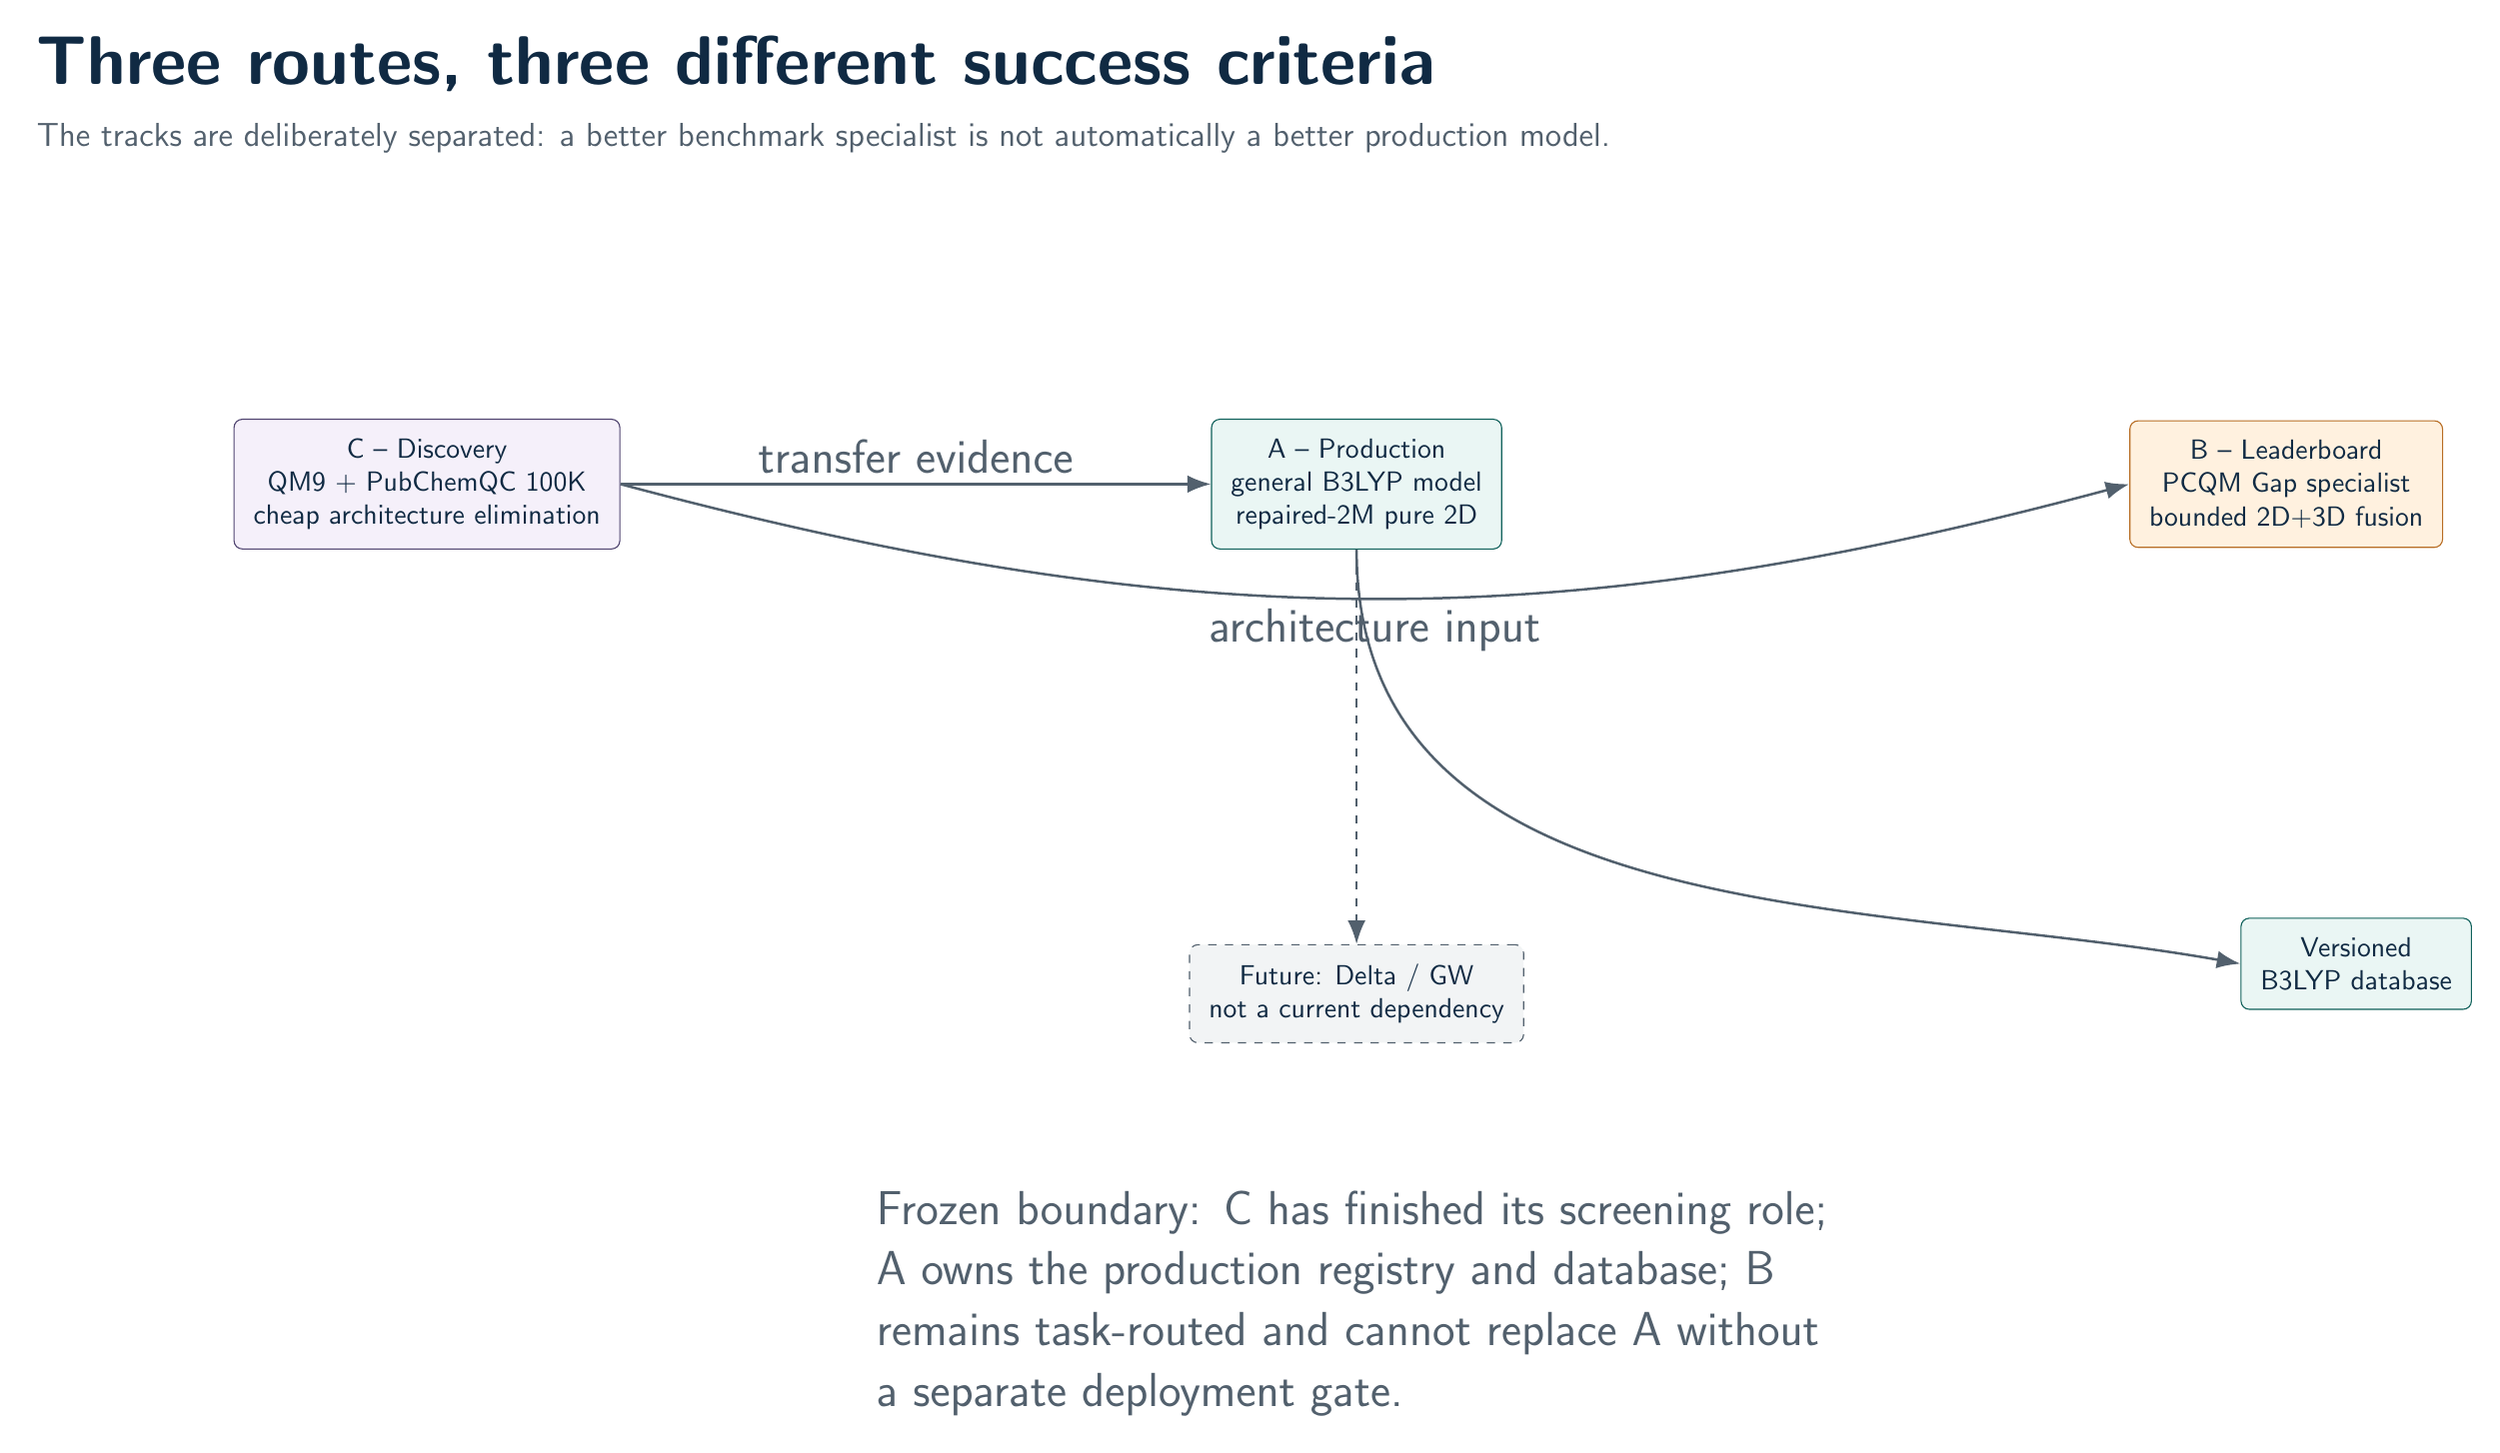
\begin{tikzpicture}[x=1in,y=1in]
  \node[title,anchor=west] at (0,6.85) {Three routes, three different success criteria};
  \node[subtitle,anchor=west] at (0,6.48) {The tracks are deliberately separated: a better benchmark specialist is not automatically a better production model.};

  \node[data,minimum width=3.1cm,minimum height=1.15cm] (c) at (2.0,4.75) {C -- Discovery\\QM9 + PubChemQC 100K\\cheap architecture elimination};
  \node[model,minimum width=3.1cm,minimum height=1.15cm] (a) at (6.65,4.75) {A -- Production\\general B3LYP model\\repaired-2M pure 2D};
  \node[specialist,minimum width=3.1cm,minimum height=1.15cm] (b) at (11.3,4.75) {B -- Leaderboard\\PCQM Gap specialist\\bounded 2D+3D fusion};

  \draw[arrow] (c.east) -- node[above,note] {transfer evidence} (a.west);
  \draw[arrow] (c.east) to[out=-15,in=-165] node[below,note] {architecture input} (b.west);
  \node[model,minimum width=2.35cm,minimum height=0.95cm] (db) at (11.65,2.35) {Versioned\\B3LYP database};
  \draw[arrow] (a.south) to[out=-90,in=170] (db.west);
  \node[future,minimum width=3.1cm,minimum height=0.9cm] (future) at (6.65,2.2) {Future: Delta / GW\\not a current dependency};
  \draw[dashedarrow] (a.south) -- (future.north);

  \node[note,text width=12.2cm] at (6.65,0.65) {Frozen boundary: C has finished its screening role; A owns the production registry and database; B remains task-routed and cannot replace A without a separate deployment gate.};
\end{tikzpicture}
\end{document}
